\documentclass{beamer}  
\usepackage{amsmath}
\usepackage{graphicx}
\usepackage{url}
\usepackage{listings}
\usepackage{fancyvrb}
\usepackage[T1]{fontenc}
\usepackage{hyperref}
\mode<presentation>
{ \usetheme{Warsaw} }
\title{Greedy, Divide and Conquer
}

\author{League of Programmers}
\institute{ACA, IIT Kanpur}
\date{October 22, 2012}
 
\AtBeginSection[]  % "Beamer, do the following at the start of every section"
{
\begin{frame}<beamer> 
\frametitle{Outline} % make a frame titled "Outline"
\tableofcontents[currentsection]  % show TOC and highlight current section
\end{frame}
}

\begin{document}
%----------- titlepage ----------------------------------------------%
\begin{frame}
  \titlepage
\end{frame}

\section{Greedy Algorithms}
%----------- slide --------------------------------------------------%
\begin{frame}[<+->]{Greedy Algorithms}
\begin{itemize}
  \item Greedy algorithms are generally used in optimization problems
  \item There is an optimal substructure to the problem
  \item Greedy Algorithms are algorithms that
  \begin{itemize}
  \item try to maximize the function by making greedy choice at all points. In other words, we   do at each step what seems best without planning ahead
  \item ignores future possibilities (no planning ahead)
  \item never changes choice (no backtracking)
  \end{itemize}
  \item Usually O(n) or O(n lg n) Solutions.
  \item But, We must be able to prove the correctness of a greedy algorithm if we are to be sure that it works
\end{itemize}
\end{frame}

\begin{frame}{Problem}
  \begin{block}{Problem 1:}
  A family goes for picnic along a straight road. There are k hotels in their way situated at distances $d_1$,$d_2$ \ldots $d_k$ from the start. The last hotel is their destination. The can travel at most L length in day. However, they need to stay at a hotel at night. Find a strategy for the family so that they can reach hotel k in minimum number of days.
  \end{block}
\end{frame}

\begin{frame}{Problem}
  \begin{block}{Solution:}
  The first solution that comes to mind is to travel on a particular day as long as possible, i.e. do not stop at a hotel iff the next hotel can be reached on the same day.
  \end{block}
\end{frame}

\begin{frame}{Problem}
  \begin{block}
  {\bf Proof:}
  Proof strategy 1 for greedy algorithms:\\
  \begin{itemize}
  \item Greedy solution stays ahead
  \item Suppose there is a better solution which stops at hotels $i_1$ < $i_2$ \ldots $i_r$ and greedy solution stops at $j_1$ < $j_2$ \ldots $j_s$ and $r<s$.
  \item Consider the first place where the two solutions differ and let that index be p. Clearly $i_p$ < $j_p$
  \item On a given day when non greedy solution starts from hotel $i_q$<$j_q$, non greedy solution cannot end up ahead of greedy solution.
  \item Therefore Greedy solution stays ahead
  \end{itemize}
  \end{block}
\end{frame}

\begin{frame}{Problem}
  \begin{block}{Problem 2:}
  There are n processes that need to be executed. Process i takes a preprocessing time $p_i$ and time $t_i$ to execute afterwards. All preprocessing has to be done on a supercomputer and execution can be done on normal computers. We have only one supercomputer and n normal computers. Find a sequence in which to execute the processes such that the time taken to finish all the processes is minimum.
  \end{block}
\end{frame}

\begin{frame}{Problem}
  \begin{block}{Solution:}
  Sort in descending order of $t_i$ and execute them. At least this is the solution for which no counterexample is available.
  \end{block}
\end{frame}

\begin{frame}{Problem}
  \begin{block}{Proof:}
  \begin{itemize}
  \item Let there be any other ordering $\sigma$(1),$\sigma$(2)\ldots $\sigma$(n) such that $t\sigma$(i) < t$\sigma$(i+1) for some i.
  \item Prove that by executing $\sigma$(i+1) before $\sigma$(i), we will do no worse.
  \item Keep applying this transformation until there are no inversions w.r.t. to t. This is our greedy solution.
  \end{itemize}
  \end{block}
\end{frame}

\begin{frame}{Problem}
  \begin{block}{Problem 3:}
  A thief breaks into a shop only to find that the stitches of his bag have become loose. There are N items in the shop that he can choose with weight W[i] and value V[i]. The total weight that the bag can carry is W. How should he choose the items to maximize the total value of the things he steals?
  \end{block}
\end{frame}

\section{Divide and Conquer}
\begin{frame}[<+->]{Divide and Conquer}
  \begin{block}{}
  \begin{itemize}
  \item Suppose P(n) is the problem we are trying to solve, of size n\\
  \item We can solve P(n) directly, for sufficiently small n\\
  \item Divides the problem P(n) into subproblems\\
  \begin{center}$P_1$($n_1$); $P_2$($n_2$); : : : ; $P_k$($n_k$)\end{center} for some constant k
  \item Combine the solutions for $P_i$($n_i$) ($1 \leq i \leq k$) to solve P(n)
  \end{itemize}
  \end{block}
\end{frame}

\begin{frame}{Problem}
  \begin{block}{Problem 1:}
  \begin{itemize}
  \item {\bf Merge-sort is divide-n-conquer.}
  \item Analysis of merge-sort.
  \begin{center}$T(n) \leq 2T(n/2) + n$\end{center}
  \item Problem- Find number of inversions by modifying code for merge-sort slightly.
  \end{itemize}
  \end{block}
\end{frame}

\begin{frame}{ClosestPair Problem}
  \begin{block}{Closest Pair of points}
    Given N points in a plane, find the pair of points that are closest to each other.
  \end{block}
\end{frame}

\begin{frame}[<+->]{ClosestPair Problem}
  \begin{columns}[t]
    \begin{column}{0.5\textwidth}
      \vspace{10mm}
      \begin{figure}
	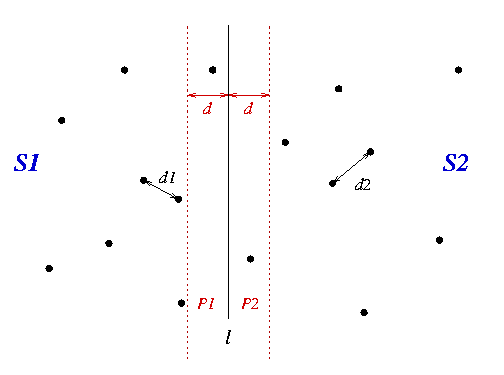
\includegraphics[scale=0.30]{figure21.png}
	\caption{1}
      \end{figure}
    \end{column}
    \begin{column}{0.5\textwidth}
      \begin{itemize}
	\item First sort the points in increasing order of X coordinate.
	\item Divide the plane into two halves with equal number of points P1 and P2.
	\item Let d1 be the minimum distance between closest pair in the P1 and similarly d2 in P2.
	\item d1$:$ minimum distance of P1
	\item d2$:$ minimum distance of P2
	\item d $\leq$ min\{d1, d2\}.
      \end{itemize}
    \end{column}
  \end{columns}
\end{frame}

\begin{frame}[<+->]{ClosestPair Problem}
  \begin{itemize}
  \item Now, region of interest is the band of 2d around the dividing line.
  \item \alert{But, In fact, all of the points could be in the strip! This is disastrous, because we would have to compare $n^2$ pairs of points to merge the set, and hence our divide\-and\-conquer algorithm wouldn't save us anything in terms of efficiency.}
  \end{itemize}
\end{frame}

\begin{frame}{ClosestPair Problem}
  \begin{columns}[t]
    \begin{column}{0.3\textwidth}
      \vspace{10mm}
      \begin{figure}
	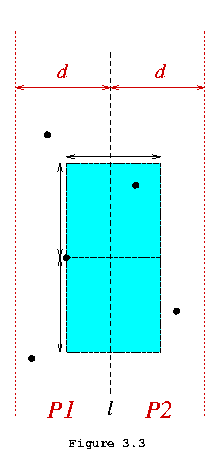
\includegraphics[scale=0.30]{figure22.png}
	\caption{2}
      \end{figure}
    \end{column}
    \begin{column}{0.7\textwidth}
      \only<2>{Thankfully, we can make another life saving observation at this point. For any particular point p in one strip, only points that meet the following constraints in the other strip need to be checked$:$
      \begin{enumerate}
	\item Those points within d of p in the direction of the other strip
	\item Those within d of p in the positive and negative y directions
      \end{enumerate}
      because points outside of this bounding box cannot be less than d units from p.\\}
      \begin{itemize}
	\only<3->{\item It just so happens that because every point in this box is at least d apart, there can be \alert{at most six points within it}.}
	\only<4->{\item Now we don't need to check all $n^2$ points. All we have to do is sort the points in the strip by their y-coordinates and scan the points in order, checking each point against a maximum of 6 of its neighbors.}
	\only<5->{\item This means at most \alert{$6*n$} comparisons are required to check all candidate pairs.}
      \end{itemize}
    \end{column}
  \end{columns}
\end{frame}

\begin{frame}[<+->]{ClosestPair Problem}
  \begin{block}{Summary}
  \begin{enumerate}
    \item Divide the set into two equal sized parts by the line l, and recursively compute the minimal distance in each part.
    \item Let d be the minimal of the two minimal distances.
    \item Eliminate points that lie farther than d apart from l
    \item Sort the remaining points according to their y-coordinates
    \item Scan the remaining points in the y order and compute the distances of each point to its five neighbors.
    \item If any of these distances is less than d then update d.
  \end{enumerate}
  \end{block}
\end{frame}

\begin{frame}[<+->]{ClosestPair Problem}
  \begin{block}{Analysis}
  Steps 2-6 define the merging process which must be repeated log(n) times because this is a divide and conquer algortithm:
  \begin{itemize}
    \item Step 2 takes O(1) time
    \item Step 3 takes O(n) time
    \item Step 4 is a sort that takes O(nlogn) time
    \item Step 5 takes O(n) time (as we saw in the previous section)
    \item Step 6 takes O(1) time
  \end{itemize}
  \only<7->{Hence the merging of the sub-solutions is dominated by the sorting at step 4, and hence takes O(nlogn) time.\\}
  \only<8->{This must be repeated once for each level of recursion in the divide-and-conquer algorithm, hence the whole of algorithm ClosestPair takes \alert{O(logn*nlogn) = O(n$log^2n$)} time.}
  \end{block}
\end{frame}

\begin{frame}{ClosestPair Problem}
  \begin{block}{Improving the Algorithm}
    \only<1>{We can improve on this algorithm slightly by reducing the time it takes to achieve the y-coordinate sorting in Step 4. This is done by asking that the recursive solution computed in Step 1 returns the points in sorted order by their y coordinates. This will yield two sorted lists of points which need only be merged in Step 4 in order to yield a complete sorted list.} \only<2->{Hence the revised algorithm involves making the following changes:}
    \begin{itemize}
      \only<3->{\item Step 1: Divide the set into\dots, and recursively compute the distance in each part, returning the points in each set in sorted order by y-coordinate.}
      \only<4->{\item Step 4: Merge the two sorted lists into one sorted list in O(n) time. Hence the merging process is now dominated by the linear time steps thereby yielding an O(nlogn) algorithm for finding the closest pair of a set of points in the plane.}
    \end{itemize}
  \end{block}
\end{frame}

\begin{frame}{Divide and Conquer}
  \begin{block}{When to use divide and conquer}
    \only<2->{Divide and conquer works well when:}
    \begin{itemize}
      \only<3->{\item Divide step produces a constant number of subproblems}
      \only<4->{\item The subproblems may be solved independently}
      \only<5->{\item The size of each subproblem is much smaller than the original}
    \end{itemize}
    \only<6->{Divide and Conquer is a bad choice when:}
    \begin{itemize}
      \only<7->{\item There are too many subproblems}
      \only<8->{\item The subproblems are not independent}
      \only<9->{\item The subproblems are too large}
    \end{itemize}
  \end{block}
\end{frame}

\section{Binary Search}
\begin{frame}[<+->]{Binary Search}
  \begin{block}{}
  {\bf Problem: Finding a value in a sorted sequence}\\
  For example, find 55 in the sequence
  \begin{center}0, 5, 13, 15, 24, 43, 55, 65, 72, 85, 96\end{center}
  \only<2->{What is the time complexity?\\}
  \only<3->{\alert{At each step, we are discarding half of the array.}}
  \end{block}
\end{frame}

\begin{frame}[<+->]{Binary Search}
  \begin{block}{Code}
    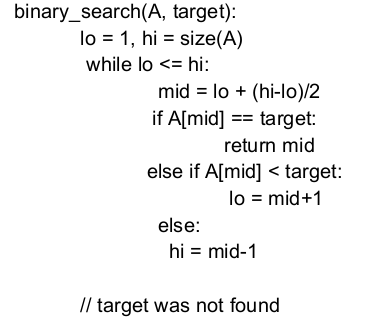
\includegraphics[scale=0.45]{figure23.png}
  \end{block}
\end{frame}

\begin{frame}{Problem}
  \begin{block}{}
    In a building with 100 (=n) storeys a person is required to find starting from which floor an egg if thrown to the ground will be broken. He has been given just 2(=m) eggs for this task. All he can do is to go to certain storeys and throw his egg and record whether the egg broke or not. Assume that for each storey, an egg will either always break or will never break. Since, climbing stairs (there's no lift!), throwing eggs and going downstairs again to check whether the egg broke or not and to take the egg again to the next floor being checked can be a tiring process, devise a strategy following which the person will find the required storey having after minimum number of throws
  \end{block}
\end{frame}

\begin{frame}{Generalization}
  \begin{block}{Extending the idea of Problem 1}
    The same algorithm described above on any monotonic function f whose domain is the set of integers. The only difference is that we replace an array lookup with a function evaluation: we are now looking for some x such that f(x) is equal to the target value
  \end{block}
\end{frame}

\begin{frame}{Problem}
  \begin{block}{Problem:}
  \href{http://code.google.com/codejam/contest/1150485/dashboard\#s=p1&a=1}{CodeJam}
  \end{block}
\end{frame}

\section{Problems}

\begin{frame}{Problems}
Links:
\begin{enumerate}
\item \url{http://spoj.pl/problems/BALIFE}
\item \url{http://www.spoj.pl/problems/PANCAKES}
\item \url{http://spoj.pl/problems/AGGRCOW}
\item \url{http://spoj.pl/problems/ARRANGE}
\item \url{http://www.spoj.pl/problems/BIASED}
\item \url{http://www.spoj.pl/problems/DONALDO}
\item \url{http://www.spoj.pl/problems/PIE}
\item \url{http://www.spoj.pl/problems/CISTFILL}
\end{enumerate}
\end{frame}

\begin{frame}{Acknowledgements}
  \begin{block}{}
    Image Credits:
      \href{http://www.cs.mcgill.ca/~cs251/ClosestPair/ClosestPairDQ.html}{http://www.cs.mcgill.ca/~cs251/ClosestPair/ClosestPairDQ.html}
  \end{block}
\end{frame}

\end{document}
